\chapter{Reference Coverage and Granularity}

This chapter is based on the following publications.
\begin{quote}
\fullcite{Saier2022ULITE}\\
\fullcite{Saier2023unarXive}
\end{quote}

% \begin{abstract}
% Analyses and applications based on bibliographic references are of ever increasing importance. However, reference linking methods described in the literature are only able to link around half of the references in papers. To improve the quality of reference linking in large scholarly data sets, we propose a blocking-based reference linking approach that utilizes a rich set of reference fields (title, author, journal, year, etc.) and is independent of a target collection of paper records to be linked to. We evaluate our approach on a corpus of 300,000 references. Relative to the original data, we achieve a 90\% increase in papers linked through references, a five-fold increase in bibliographic coupling, and a nine-fold increase in in-text citations covered. The newly established links are of high quality (85\% F1). We conclude that our proposed approach demonstrates a way towards better quality scholarly data.
% \end{abstract}

\section{A Blocking-Based Approach to Enhance Large-Scale Reference Linking}

\subsection{Introduction}
% % Motivation
Scholarly data is becoming increasingly important and with it its quality and coverage. Connections between publications in the form of literature references are of particular importance, as they are used as a basis for various analyses, decision making, and applications. Some examples are research output quantification~\cite{Hirsch2005}, trend detection~\cite{Chen2006}, summarization~\cite{Elkiss2008}, and recommendation~\cite{Ma2020,Faerber202x}.

% Problem
%However, in current data sets providing interlinked publications, only around half of the references contained in the original papers are linked\footnote{We use ``link[ing/ed] references'' w.r.t. to connections to cited papers rather than in-text citation markers.} to the cited publications~\cite{Lo2020,Saier2020}. This lack in coverage is especially affecting references to non-English publications~\cite{Saier2021}, which are in general underrepresented in scholarly data~\cite{Vera-Baceta2019,Liu2019,Moed2018,Moskaleva2019} along with publications in the humanities~\cite{Colavizza2019,Kellsey2004}.
However, reference linking methods\footnote{We use ``link[ing/ed] references'' w.r.t. to connections to cited papers rather than in-text citation markers.} described in the literature are only able to link around half of the references contained in the original papers to the cited publications~\cite{Lo2020,Saier2020}. This lack in coverage is especially affecting references to non-English publications~\cite{Saier2021}, which are in general underrepresented in scholarly data~\cite{Vera-Baceta2019,Liu2019,Moed2018,Moskaleva2019} along with publications in the humanities~\cite{Colavizza2019,Kellsey2004}.

We see the reason for this lack in linked references in two key shortcomings of current methods.
First, references are linked using simple string similarity measures that are often relying \emph{only} on publications' title and author information (which is not always contained in references; see Figure~\ref{fig:hardmatch}). %Note: maybe add sth. along the lines of “relying on title (and mby authors) is deemed sufficient”
Second, references are exclusively linked to a target collection of paper records---usually a large metadata set like DBLP\footnote{See \url{https://dblp.org/}.} or OpenAlex\footnote{See \url{https://openalex.org/}.}, or a set of IDs like DOIs or PMIDs. This means references to literature which is not contained in the target collection, as well as to non-source items~\cite{Chi2014}, cannot be linked (see ``?'' markers in Figure~\ref{fig:approach}).

\begin{figure}[tb]
  \centering
  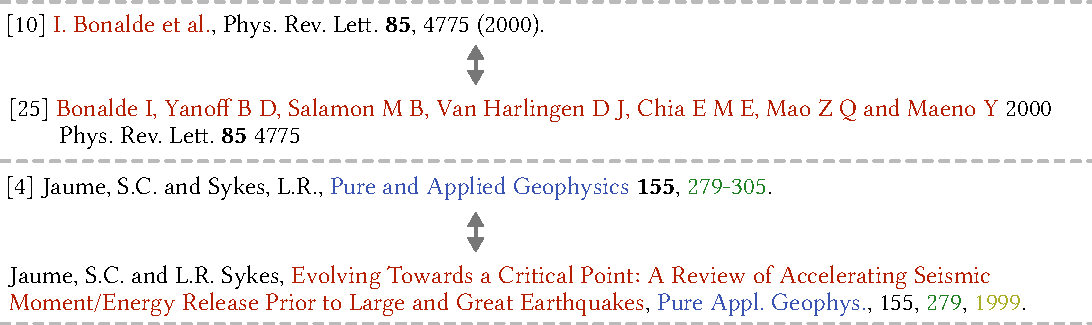
\includegraphics[width=\linewidth]{figures/ref_covgran/hardmatch_examples.pdf}
  \caption{Examples of challenging reference pairs from our evaluation that where successfully matched. \textbf{Top:} references from \texttt{arXiv:cond-mat/0503317} (no title, first author only) and \texttt{arXiv:cond-mat/0104493} (no title, all authors). \textbf{Bottom:} references from \texttt{arXiv:cond-mat/0104341} (no title, full venue, page rage, no year) and \texttt{arXiv:physics/0504218} (with title, venue abbreviation, start page only, with year).}
  \label{fig:hardmatch}
\end{figure}

\begin{figure}[tb]
  \centering
  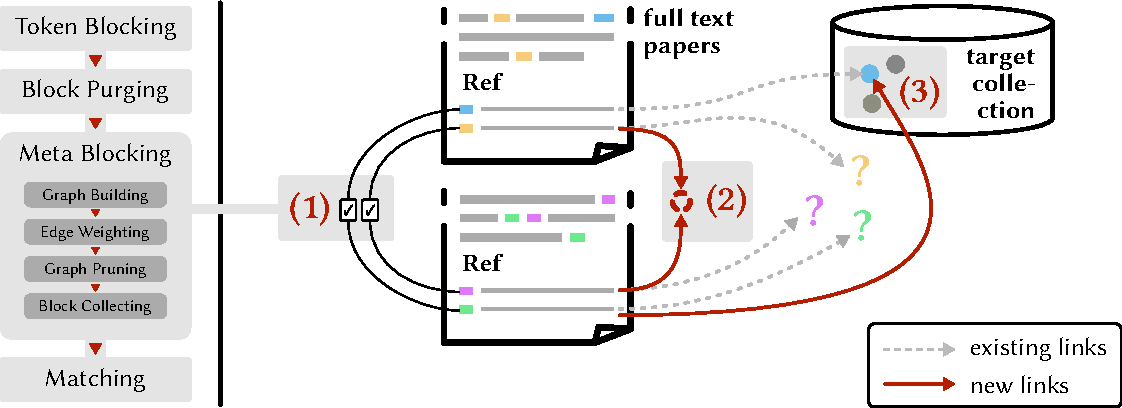
\includegraphics[width=\linewidth]{figures/ref_covgran/approach_withblocking_10pvar.pdf}
  \caption{Schematic depiction of the use case. A corpus of full text papers, where some references are already linked to a target collection (blue), and some are not (orange, pink, green). At \textbf{(1)} we apply our blocking and matching approach to identify all references that point to the same publication. In doing so, we establish new links in the form of \textbf{(2)} bibliographic coupling and \textbf{(3)} links to the target collection.}
  \label{fig:approach}
\end{figure}

%ER related work
Linking references can be seen as a task of entity resolution (ER)~\cite{Christophides2015ERdef}, which is concerned with identifying entities referring to the same object within or between large data sets. Because the task requires a one-to-one comparison between each of the involved entities, it is inherently of quadratic complexity. To make approaches scalable, entities are assigned into groups of likely matching candidates prior to comparison, a technique called blocking~\cite{Papadakis2020survey}.
While blocking-based approaches are used in the domain of scholarly data to, for example, identify duplicate paper records~\cite{Simonini2016blast,Sefid2019,Lo2020} (where information such as abstracts are used) and authors~\cite{FaerberLin2022}, they are not utilized for bibliographic references.

% Our solution
We therefore address both of the aforementioned problems with current reference linking approaches, (1)~the use of simple matching methods based on title and authors, as well as (2)~the reliance on a target collection of paper records, by proposing (1)~the use of a blocking and matching process utilizing seven reference fields (title, author, journal, year, etc.) that (2)~operates \emph{within} the set of bibliographic references of a corpus, and is thereby \emph{independent} of a target collection of papers (see marker ``(1)'' in Figure~\ref{fig:approach}).

We showcase the feasibility and benefits of our approach, implementing a pre-processing, blocking, and matching pipeline and evaluating it on a corpus containing 300,000 references.
We show that relative to the original data, our approach gives us a \textbf{90\% increase} in papers linked to the target collection, a \textbf{five-fold increase} in bibliographically coupled~\cite{Boyack2010} papers (see marker ``(2)'' in Figure~\ref{fig:approach}), and a \textbf{nine-fold increase} in in-text citation markers covered.\footnote{With the ``coverage'' of in-text citation markers we refer to markers associated with linked references, relative to markers belonging to unlinked references.} The new links are furthermore of high quality (85\% F1). This paves the way towards higher quality scholarly data, especially regarding the coverage of so far underrepresented literature and non-source items.

In summary, we make the following contributions.

\begin{itemize}
    \item We propose a blocking-based approach for matching bibliographic references that is independent of a target collection of paper records.
    \item We perform a large-scale evaluation showing that our approach results in a manifold increase in high quality reference links.
    \item We make our data and code publicly available.\footnote{See \url{https://github.com/IllDepence/ulite2022}.}
\end{itemize}

\subsection{Related Work}
Blocking-based approaches have been used in the domain of scholarly data, though to the best of our knowledge not for bibliographic references. We therefore report on (1) exemplary uses of blocking in the scholarly domain for entities other than references, and (2) approaches to linking bibliographic references using methods other than blocking.

Simonini et al.~\cite{Simonini2016blast} develop BLAST (Blocking with Loosely-Aware Schema Techniques) which adapts Locality-Sensitive Hashing. Among data sets from other domains, they also evaluate their approach for the task of linking 2,600 DBLP paper records to the ACM\footnote{See \url{https://dl.acm.org/}.} and Google Scholar.\footnote{See \url{https://scholar.google.com/}.} 
Sefid~\cite{Sefid2019} proposes several models to match paper records utilizing the papers' title, header, and citation information. The models are evaluated in three scenarios matching 1,000 paper records from CiteSeer$^x$~\cite{CiteSeerX2019} to IEEE, DBLP, and Web of Science.
Lastly, Färber et al.~\cite{FaerberLin2022} detect duplicates among 243 million author records in the Microsoft Academic Knowledge Graph~\cite{MAKG} and evaluate their approach using ORCiD IDs.

%                        GROBID | LaTeX
% Bibliography entries   27.6M  | 21.9M*
% Linked bib. entries    19.3M  |  6.8M*
%
% *The lower number of linked bibliography entries in latex parses is due to large numbers of papers (mostly in the field of physics) for which the bibliography entries are formatted without paper titles. Our linking algorithm strongly depends on titles and fails to link these entries.
Lo et al.~\cite{Lo2020} introduced the data set S2ORC, which contains 9.6 million open access papers and has recently seen extensive use in area of scholarly document processing. The authors link references to papers within their data set using a heuristic similarity measure based on n-grams and the Jaccard similarity, which only uses the paper title. Using this method, 26 million out of 50 million references  (52\%) are successfully linked. The authors report that the low number is \textit{``due to large numbers of papers (mostly in the field of physics) for which the bibliography entries are formatted without paper titles.''} Saier et al.~\cite{Saier2020} introduce unarXive, a data set created from papers' \LaTeX\ sources containing over 1 million publications. Bibliographic references in the data set are linked to the Microsoft Academic Graph~\cite{Sinha2015,Wang2019}. The linking procedure is based on string similarity of papers' titles and author information. With this procedure 17 million out of 40 million references (42\%) are successfully linked.
Lastly, CiteSeer$^x$~\cite{CiteSeerX2015,CiteSeerX2019} in another large data set containing paper records. Similar to S2ORC, references are linked to paper records within the data set itself. In the case of CiteSeer$^x$ the linking is performed through a heuristic assignment based on title and author information.  We are not aware of information on the percentage of references that are successfully linked in CiteSeer$^x$.

%ad hoc~\cite{Kokash2022}
%web services often just link to search (lmgtfy)

\subsection{Approach}

Our approach consists of the following three steps: (1) \emph{pre-processing} to convert references into a normalized, structured format, (2) \emph{blocking} to allow us to process large amounts of references, and (3) \emph{matching}. These steps are explained in more detail below.

%Our approach consists of the following three steps: (1)~\emph{pre-processing} to convert references into a normalized, structured format, (2)~\emph{blocking} to allow us to process large amounts of references, and (3)~\emph{matching} to determine references that refer to the same publication. Conceptually the steps operate on the level of (1)~single entities, (2)~blocks (sets of entities or entity pairs), and (3)~entity pairs. Below the steps are explained in more detail.

\paragraph{Pre-processing}
References as they appear in papers are hard to match for several reasons, such as the variety of citation styles, variants of author names, venue abbreviations, sparsity of information, and typing errors~\cite{Christen2012} (see Figure~\ref{fig:hardmatch}). To mitigate these issues, we pre-process references in three steps: first, we apply GROBID's~\cite{Lopez2009} reference string parsing module,\footnote{See \url{https://grobid.readthedocs.io/en/latest/Grobid-service/\#apiprocesscitation}.}\footnote{GROBID was chosen according to the results of~\cite{Tkaczyk2018}.} then we expand journal and conference abbreviations, and lastly all strings are lowercased and Unicode normalized. For the abbreviation expansion we use a mapping for 47.6k journal titles provided by JabRef\footnote{See \url{https://github.com/JabRef/abbrv.jabref.org}.} and 2.6k conference titles crawled from various web sources. Following~\cite{Koo2011} we select seven reference fields for the blocking step: title, author, year, volume, journal, booktitle, and pages.

\paragraph{Blocking}
%Blocking is an essential technique in the field of ER~\cite{Papadakis2020survey} used to reduce the number of necessary one-to-one comparisons in or between large data sets. 
%Following~\cite{Papadakis2016}, we build our pipeline with two blocking components, namely  (1)~block building, and (2)~block cleaning. In the subsequent matching step a third component, (3)~comparison cleaning, is applied. As shown in Figure~\ref{fig:approach}, we use token blocking, block purging, and meta-blocking respectively for each of the three steps.
Following~\cite{Papadakis2016}, we build our blocking pipeline from components for (1) block building, (2) block cleaning, and (3) comparison cleaning. As shown in Figure~\ref{fig:approach}, we use token blocking, block purging, and meta-blocking respectively for each of the steps.

\emph{Token blocking} is chosen for the block building step because it is schema-agnostic and therefore robust against the varying level of information contained in or missing from bibliographic references. In this step, references are assigned to blocks based on all tokens (i.e., words) contained in the identified and normalized reference fields. As a result, references at this point are associated with multiple blocks, which leads to a high level of redundancy.

\emph{Block purging}~\cite{Papadakis2011blockpurging} removes oversized blocks based on a comparison cardinality metric, which we determine heuristically and set it to 0.01. Intuitively, the removed blocks originate from common tokens, meaning that matched reference strings within them are highly likely to also share smaller blocks. Purging therefore reduces the number of overall comparisons with minimal effect on the final result quality.

\emph{Meta-blocking}~\cite{Papadakis2014}, our comparison cleaning step, reduces unnecessary comparisons within blocks by generating a weighted graph of entities (references in our case) based on their shared blocks, removing edges based on a pruning scheme, and lastly creating a new block collection based on the reduced graph. For both the weighting and the pruning of edges several schemes exist. In Section~\ref{sec:eval} we describe how we determined the most suitable combination of schemes for our use case. Here, we briefly mention the schemes involved. Available graph weighting schemes include the Common Blocks Scheme (CBS), the Enhanced Common Blocks Scheme (ECBS), the Aggregate Reciprocal Comparisons Scheme (ARCS), and the Jaccard Scheme (JS). For graph pruning, we consider Cardinality Node Pruning (CNP), which relies on cardinality to select the top edges for each node, as well as Weight Edge Pruning (WEP), which removes edges based on their assigned weight.

% \emph{Meta-blocking}~\cite{Papadakis2014}, our comparison cleaning step, reduces unnecessary comparisons within blocks and consists of four sub-steps: graph building, edge weighting, graph pruning, and block collecting.

% In the \emph{graph building} step, the block collection is transformed in a blocking graph, where an entity (i.e. reference string) is represented as a node, and the co-occurrence of two entities in a common block is conveyed by an edge connecting them. Since a new edge is only created for a pair of entities that hasn’t appear yet. If a pair of entities share more than one block, they will only be connected by one edge and will not appear repeatedly in the blocking graph. 

% The information conveyed through the number of blocks shared by a pair of entities is entailed in the weight of the edge between the pair, which is determined in the \emph{edge weighting} step relying on a weighting scheme. There are five weighting schemes available: (1)	Aggregate Reciprocal Comparisons Scheme(ARCS), (2)	Common Blocks Scheme(CBS), (3) Enhanced Common Blocks Scheme(ECBS), (4)	Jaccard Scheme(JS), and (5)	Enhanced Jaccard Scheme(EJS).

% In the next step, \emph{graph pruning} depends on a pruning scheme to prune the weighted blocking graph. There are four pruning schemes available: (1)    Weight Edge Pruning(WEP), examines all the edges in the blocking graph and remains those, whose weight reaches a minimum edge weight, (2)    Cardinality Edge Pruning(CEP), only those top edges with the highest weight in the blocking graph are remained according to a cardinality threshold, (3)    Weight Node Pruning(WNP), set a local weight threshold for each node to discard edges that linked to the node, and (4)    Cardinality Node Pruning(CNP), relies on a cardinality threshold to select the top edges for each node from all the edges that linked to the node.

% As the last step of blocking, \emph{block collecting} creates a new block collection with all remaining reference strings based on the pruned blocking graph.

\paragraph{Matching}

To determine which references within a block refer to the same publications, we utilize a weighted average of Jaccard similarities across our seven reference fields. Based on~\cite{Foufoulas2017} as well as preliminary experiments, we set the weights for title, author, journal, booktitle, year, volume, and pages to $8$, $6$, $5$, $5$, $3$, $3$, and $2$ respectively, and set the threshold for a match to $0.405$.

% \paragraph{Matching}
% After blocking, whether reference strings within the same blocks match the same document or not should be determined. Among various similarity measures~\cite{Christen2012}, token-based metrics are better suited to comparing long strings involving multiple tokens. We apply Jaccard similarity metric for computing similarity between reference strings,which measures the percentage of common tokens shared by both strings and is calculated as the common tokens within both strings divided by the number of all distinct tokens in both strings.  

% Based on~\cite{Foufoulas2017} and preliminary experiments, we assign different weight to different metadata fields, and compute the similarity for each metadata field separately to avoid mismatch when the same token appears in different fields and at the same time, to consider the different importance of different metadata fields. 
% Taking the coverage of metadata fields into account, we calculate the value of $SumSim$ by adding the weighted Jaccard similarity value of all the selected fields together.
% \begin{equation}
%   \begin{aligned}
%   {SumSim}=8\times{sim}_{Jaccard}(title)+6\times{sim}_{Jaccard}(author)+5\times{sim}_{Jaccard}(journal)\\
%   +5\times{sim}_{Jaccard}(booktitle)+3\times{sim}_{Jaccard}(year)\\
%   +3\times{sim}_{Jaccard}(volume)+2\times{sim}_{Jaccard}(pages)
%   \end{aligned}
% \end{equation}

% In order to ensure that the value of final similarity falls in the interval [0,1], the final similarity between a pair of reference strings $p_j$ and $p_k$ is defined as the value of $SumSim(p_{j},p_{k})$ divided by the maximum value of the function $SumSim$ (i.e., $MaxVal$ below):

% \begin{equation}
%   {sim}(p_{j},p_{k})= \dfrac{{SumSim}(p_{j},p_{k})}{MaxVal}
% \end{equation}

% After calculating the similarity between all pairs in the resulting block collection, if the similarity value reaches the matching threshold (set to 0.405 based on preliminary experiments), the pair is thus recognized as a match. Otherwise, they are decided as non-match. 

\subsection{Evaluation}\label{sec:eval}

We use a large corpus of scholarly publications to perform two types of evaluations. (1)~A large-scale evaluation utilizing the corpus' existing reference links as ground truth, and (2)~a manual evaluation to also assess the correctness of newly created reference links. In the following, we describe the data used, evaluations performed, and results obtained.

\paragraph{Data}
For our evaluation we use the data set unarXive~\cite{Saier2020}. We chose this data set over similar data sets such as S2ORC~\cite{Lo2020}, because it not only contains paper's full text with annotated in-text citation markers, but also a dedicated database of all raw references in plain text. From unarXive we sample the 300,000 most recent references to conduct our evaluation. The 300,000 references originate from 9,917 papers from the disciplines of physics (7,347), mathematics (1,686), computer science (789), and other STEM fields (95). The publications cited through the references cover publication years from 1743 up to 2020. Four examples of references used in the evaluation are shown in Figure~\ref{fig:hardmatch}.

% \paragraph{Result}
% As a first step, token blocking generates 116,826 blocks in total with a minimum size of 2 and a maximum size of 70,372. 
% % mention through a heuristic attempt of different purging thresholds?
% In the blocking purging step, the purging threshold is calculated as 0.01. In consequence, the maximum block size is 22 and the number of comparisons after block purging is 16,585,773.
% Since meta-blocking involves five weighting schemes as well as four pruning algorithms, there exists 20 different combinations in total. 



\paragraph{Large-Scale Evaluation}

%Common Blocks Scheme(CBS)
%Enhanced Common Blocks Scheme(ECBS)
%Aggregate Reciprocal Comparisons Scheme(ARCS)
%Jaccard Scheme(JS)
%  (Enhanced Jaccard Scheme(EJS))

%Cardinality Node Pruning (CNP)
%Weight Edge Pruning (WEP)
%  (Cardinality Edge Pruning (CEP))
%  (Weight Node Pruning (WNP))

%Pair Completeness (PC)
%Pairs Quality (PQ)
%Reduction Ratio (RR)

\begin{table*}
   \caption{Performance of five graph weighting and graph pruning scheme combinations for meta-blocking.}
   \label{tab:evaluation}
   \begin{small}
   \begin{threeparttable}
   \begin{tabular}{ccccccc}
     \toprule
     Weighting scheme & Pruning scheme & \#Comparisons & \#Matches & RR\tnote{1} \ (\%) & PC\tnote{2} \ (\%) & PQ\tnote{3} \ (\%) \\
     \midrule
     CBS\tnote{4} & CNP\tnote{8} & 39,050 & 3,053 & 99.96 & 54.47 & 7.82\\
     ECBS\tnote{5} & CNP & 39,050 & 3,201 & 99.96 & \textbf{57.11} & \textbf{8.20}\\
     ARCS\tnote{6} & CNP & 39,050 & 2,890 & 99.96 & 51.56 & 7.40\\
     ARCS & WEP\tnote{9} & 24,175 & 1,285 & \textbf{99.98} & 22.93 & 5.32\\
     JS\tnote{7} & WEP & 42,919 & 2,272 & 99.96 & 40.54 & 5.29\\
   \bottomrule
 \end{tabular}
    \begin{footnotesize}
    \begin{tablenotes}
      \item[] \textit{Metrics:} \footnotemark[1]Reduction Ratio, \footnotemark[2]Pair Completeness, \footnotemark[3]Pairs Quality
      \item[] \textit{Weighting schemes:} \footnotemark[4]Common Blocks Scheme, \footnotemark[5]Enhanced Common Blocks Scheme, \footnotemark[6]Aggregate Reciprocal Comparisons Scheme, \footnotemark[7]Jaccard Scheme
      \item[] \textit{Pruning schemes:} \footnotemark[8]Cardinality Node Pruning, \footnotemark[9]Weight Edge Pruning
   \end{tablenotes}
   \end{footnotesize}
  \end{threeparttable}
  \end{small}
\end{table*}

Our large-scale evaluation is performed in two steps. First, we determine the most suitable configuration of graph weighting and pruning scheme for our meta-blocking step, then we apply our pipeline to the evaluation corpus and determine the number of additionally linked entities.

To chose a graph weighting and pruning scheme, we use the 13,976 references in our corpus which are are already linked to the target collection as ground truth. Following~\cite{Papadakis2014}, we select five combinations of schemes to evaluate. The combinations are evaluated using the metrics pair completeness (PC), which expresses the ratio of detected matches with respect to all true matches, pair quality (PQ), which estimates the portion of true matches within all executed comparisons in the block collection, and reduction ratio (RR), which measures the number of unnecessary comparisons that are saved through blocking. Table~\ref{tab:evaluation} shows the results of our evaluation. We achieve the best results using ECBS weighting and CNP pruning. Accordingly, we apply our pipeline with this configuration on the full evaluation corpus of 300k references, where our approach performs 496,051 comparisons after blocking and identifies 71,826 matches.

\begin{table*}
   \centering
   \caption{Number of linked papers, references, and in-text citations given in the original corpus and newly created through the application of our approach.}
   \label{tab:newlinks}
   \begin{small}
   \begin{threeparttable}
   \begin{tabular}{rccc}
     \toprule
     \ & \multicolumn{3}{c}{Linked to target collection} \\
     \midrule
     \ & \#Papers & \#Referencecs & \#In-text Citations \\
     Given & 1,590 & 13,975 & 23,707 \\
     New & 1,443 & 2,442 & 7,824 \\
     \midrule
     \ & \multicolumn{3}{c}{Linked through bibliographic coupling} \\
     \midrule
     \ & \#Papers & \#Referencecs & \#In-text Citations \\
     Given & - & - & - \\
     New & 8,895 & 53,940 & 219,630 \\
     \midrule
     \ & \multicolumn{3}{c}{Combined (linked in either way)\tnote{1}} \\
     \midrule
     \ & \#Papers & \#Referencecs & \#In-text Citations \\
     Given & 1,590 & 13,975 & 23,707 \\
     New & 8,931 & 55,197 & 227,454 \\
   \bottomrule
 \end{tabular}
    \begin{footnotesize}
    \begin{tablenotes}
      \item[1] Note that the combined entity counts are not simply the sum of the numbers above, because a single entity can be linked in both ways.
  \end{tablenotes}
   \end{footnotesize}
  \end{threeparttable}
  \end{small}
\end{table*}

%As shown earlier in Figure~\ref{fig:approach}, we can use the matches identified by our pipeline to create two types of new links. First, new links to the target collection (see marker ``(3)'' in Figure~\ref{fig:approach}), and second, links between references created through bibliographic coupling (see marker ``(2)'' in Figure~\ref{fig:approach})
As shown earlier in Figure~\ref{fig:approach}, we can use the matches identified by our pipeline to create two types of new links. First, new links to the target collection, and second, links between references created through bibliographic coupling. New links to the target collection are established whenever a reference with no existing link is matched to a reference with an existing link (see marker ``(3)'' in Figure~\ref{fig:approach}). In cases where neither of the references in a match have an existing link, we create a bibliographic coupling (see marker ``(2)''  in Figure~\ref{fig:approach}).
In Table~\ref{tab:newlinks} we show on the level of papers, references, and in-text citations how many links were already given in our corpus and how many new links we are able to establish. Regarding links to the target collection, we are able to link \emph{1,443 new papers} (90.75\% increase) through \emph{2,442 references} (17.47\% increase), which are connected to \emph{7,824 in-text citation markers} (33.00\% increase). As for bibliographic coupling, we connect \emph{8,895 papers} through \emph{53,940 references} connected to \emph{219,630 in-text citation markers}. Comparing the number of given links to the combined number of new links, we see a 90\% increase in papers linked to the target collection, a five-fold increase in bibliographically coupled papers, and a nine-fold increase in in-text citation markers covered.

% # ## increase
% # (1) citation graph (newly linked to the MAG)
% # - papers:             1,590 + 1,443 -> 90.75% increase
% # - references:         13,975 + 2,442 -> 17.47% increase
% # - in-text markers:    23,707 + 7,824 -> 33.00% increase
% # (2) couplings (not linked to MAG, but linked to each other)
% # - papers:             1,590 vs 8,895 -> 5.59 times of linked
% # - references:         13,975 vs 53,940 -> 3.86 times of linked
% # - in-text markers:    23,707 vs 219,630 -> 9.26 times of linked
% #
% # (3) connected (=resolved or coupled =both of the above)
% # - papers:             1,590 vs 8,931 -> 5.62 times of linked
% # - references:         13,975 vs 55,197 -> 3.95 times of linked
% # - in-text markers:    23,707 vs 227,454 -> 9.59 times of linked 

\paragraph{Manual Evaluation}
To assess the quality of our newly linked references, we take a random sample of 500 reference comparisons from the matching procedure and manually verify if our approach correctly labeled each pair as a match or non-match. This is done by inspecting both original reference strings (prior to pre-processing) and determining whether they refer to the same publication or not. Because in some disciplines such as physics it is common to see references without a title given, this process involves looking up and verifying publications' details online.\footnote{For further details see \url{https://github.com/IllDepence/ulite2022/tree/master/5_manual_evaluation}.} Examples of two reference pairs are shown in Figure~\ref{fig:hardmatch}. Comparing our predicted matches with the manually established ground truth, we measure a precision of 93.20\% and a recall of 79.34\%. Accordingly the F1-score is 85.71\%.
This shows us that our newly established links are of good quality, suggesting our approach facilitates the creation of more accurate scholarly data and, accordingly, higher quality analyses and downstream applications based scholarly data sets.
%This shows us that most of our newly established links are correct and that the number of missed links is (false negatives) is not very high.\footnote{Note that, due to the nature of our evaluation, the recall value concerns comparisons \emph{within} blocks. This means further missing links for matching references which were not placed together in any block can exist. An evaluation is unfortunately only feasible using comparisons within blocks rather than any random pairs of references in the corpus, because in the latter case the chances are very low that a random sample contains any reference pairs which were considered after blocking.}

\subsection{Discussion and Future Work}
To improve the quality of reference linking in large scholarly data sets, we proposed a blocking-based reference linking approach that is independent of a target collection of paper records. In a large-scale evaluation, we first determined the most suitable meta-blocking scheme for our particular application case. Subsequently applying our approach to a corpus of 300,000 references, we saw a manifold increase in linked papers, references, and in-text citation markers. The newly established links are of high precision and have a high recall, which we confirmed through a manual evaluation on a sample of our results. This demonstrates the benefits and quality of our approach.

Key limitations of the work presented are (1)~the size and discipline coverage of the evaluation corpus, (2)~the usage of a comparatively basic blocking technique, and (3)~the lack of a thorough evaluation of time performance.

In the future we want to address these points by expanding our work through using more advanced blocking methods such as progressive blocking~\cite{Simonini2019,Galhotra2021}, using larger evaluation corpora such as the whole unarXive data set, including data from more diverse disciplines such as the humanities, and evaluating the time performance of our approach.
%Because in our evaluation corpus references are linked to in-text citation markers in the paper full texts, we furthermore plan to explore possible application scenarios using the full text such as citation context analysis for non-source items.
Because references in our evaluation corpus are linked to in-text citation markers, we furthermore plan to explore application scenarios utilizing the paper full texts. %, such as citation context analysis for non-source items.

% Discussion:
% - Limitations:
%    - not full unarXive corpus
%    - current approach too slow
%    - only evaluated in STEM area
% - Impact:
%    - analyses (more complete citation graph, bibl. coupling of non-source items, ...)
% Future work:
% - More recent blocking/matching approach
% - include target collection into blocking&matching
%   (mby two-step s.t. from b&m in refs a "canonical representation" emerges)
% - whole unarXive corpus
% - other corpora (esp. humanities)

\subsection*{Author Contributions}  % cf. https://casrai.org/credit/
Tarek Saier: Conceptualization, Data curation (support), Formal analysis, Investigation (support), Methodology (support), Software (final evaluation), Visualization, Supervision, Writing -- original draft (lead), Writing -- review \& editing. Meng Luan: Data curation, Formal analysis, Investigation, Methodology, Software, Writing -- original draft (support). Michael F{\"a}rber: Supervision, Writing -- review \& editing.
